%=========================================================================
% (c) 2011, 2012 Josef Lusticky <xlusti00@stud.fit.vutbr.cz>

\chapter{NTP client in Contiki OS}
%\!Distinguish between TIME and CLOCK

For implementation of a reasonably useful NTP client
operating system must meet conditions listed in appendix~\ref{app:requirements}.
The main problem for NTP client implementation in Contiki is a total
lack of time support.
Not only no common interface availability but also
almost no platform-specific code has been implemented towards time support yet.
Contiki provides basic clock interface particularly for use of timers though.
This interface is is common to for all supported platforms, but the particular implementation
is platform specific.

Another deal is possible packet loss if communication uses UDP on transport layer.
The reason while this can often happen is explained in section~\ref{sec:contiki-uip}.

For developing and testing Contiki NTP client the AVR Raven platform with CPU ATmega1284P was used.
How to get a working setup with Contiki on this platform is described in
%%% CHECK THIS %%%
docs/setup.pdf file on the CD enclosed to this thesis.
%%% CHECK THIS %%%

\section{Clock interface}
Contiki feature a basic clock interface with a simple goal - measuring time.
This interface provides needed calls for timers and its defintion is to be found in /core/sys/clock.h file.
Specific implementations of this common interface are localed in /cpu direcory of Contiki source code.
Interface provides call for initialising CPU's clock system - clock\_init, that is automatically called during
boot sequence of Contiki.
The goal of the clock\_init call is to set up
appropriate timer/counter registers and interrupt service routines.
On AVR CPUs this call is implemented as C macro which evaluates to specific setup code for each CPU
when compiling.
The setup code is not common to all CPUs because of differencies among them - e.g. there are usually
only three Timer/Counter modules, but AVR ATmega1284P has four Timer/Counter modules.

%At least one of those is always 16 bit wide
%This extra module on AVR ATmega1284P is used for
% three vs. 3

%clock\_seconds
%CLOCK\_SECOND
This is however enough for implementing a reasonable time interface and later using it for NTP client.

% ntp interface extending the clock library, similiar to posix calls

%\!!AVR

\section{NTP values}
Unlike the RFC shows, there are no 64 bit values. %! RFC - A.4. Kernel System Clock Interface


\section{NTP client implementation}
The structures representing NTP message were borrowed from OpenNTPD NTP Unix daemon.
%They are not using the GCC extension for representing a bit field.

A client sends messages to each server with a poll interval of $2^{tau}$
seconds, as determined by the poll exponent tau.
In NTPv4, $\tau$ ranges from 4 (16 s) to 17 (36 h).

%! TODO
\section{Communication}
% IEEE 802.15.4
%as RFC~4944 written by 6lowpan working group of IETF
%made the underlaying IEEE 802.15.4 layer
%look like an IPv6 link~\cite{6lowpan} and
\begin{figure}
  \centering
  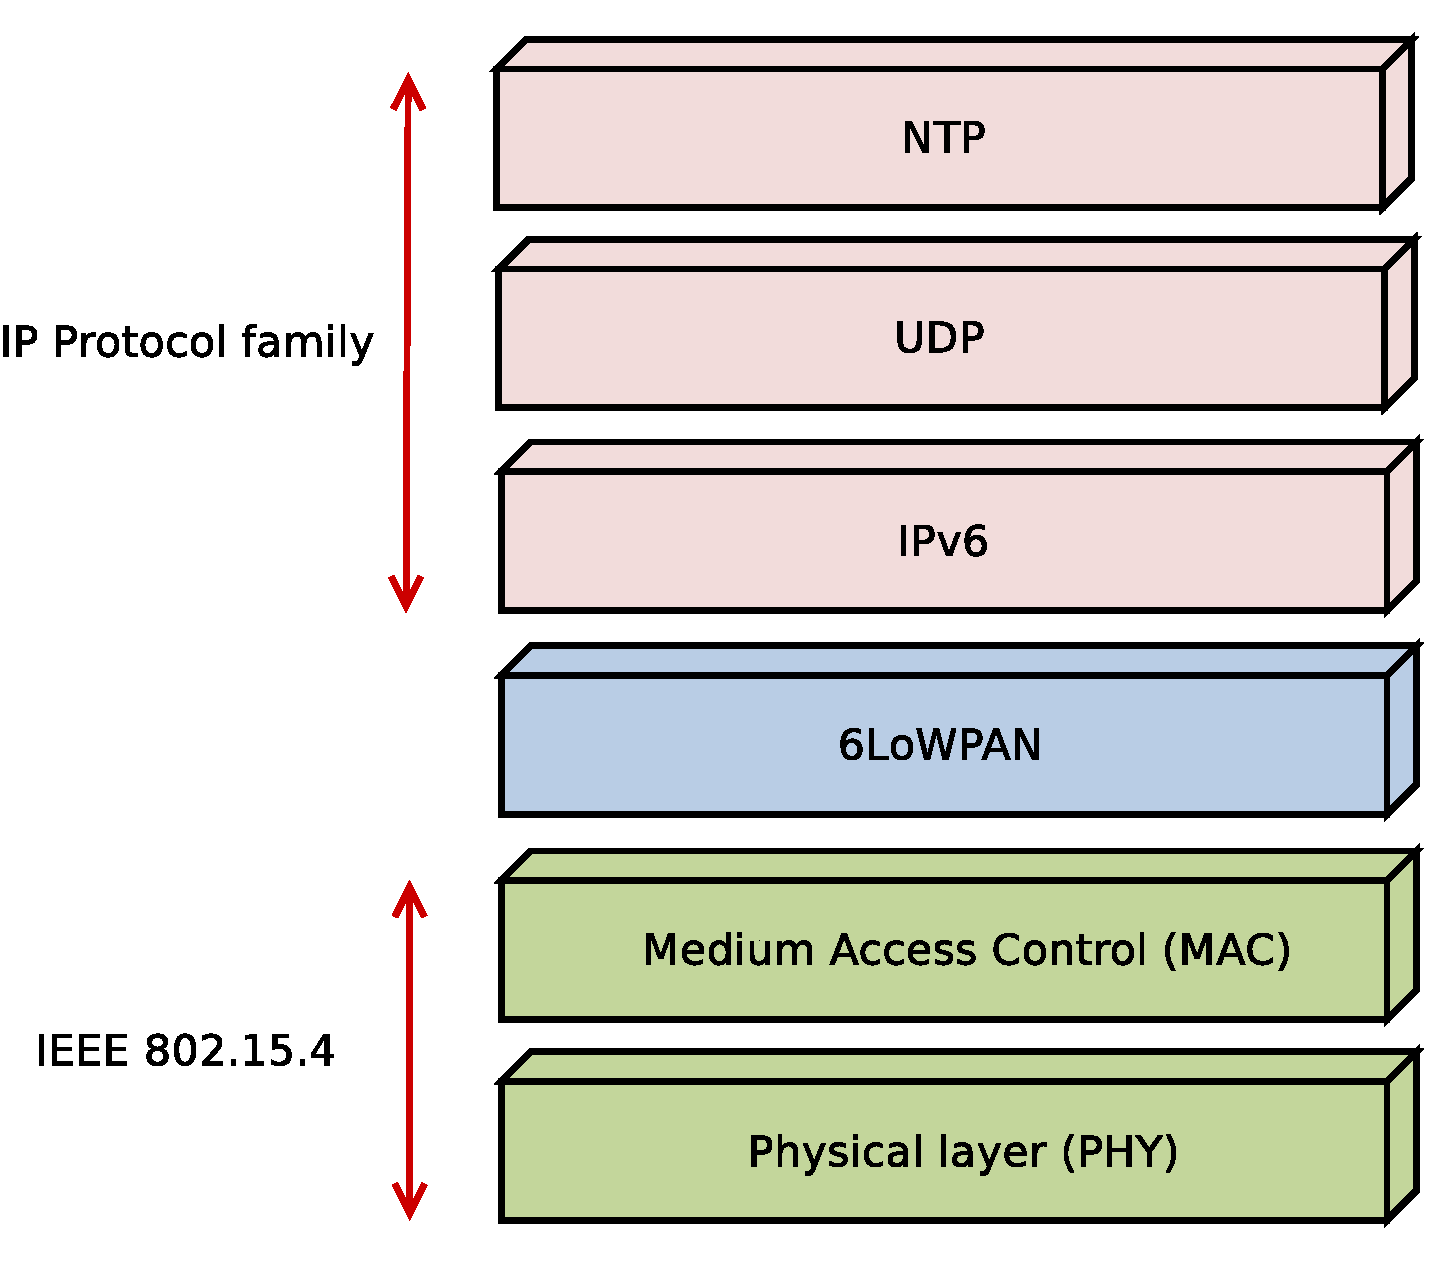
\includegraphics[width=9cm,keepaspectratio]{fig/6lowpan.pdf}
  \caption{Communication stack with 6lowpan layer}
  \label{fig:ntp-hierarchy}
  \bigskip
\end{figure}


\section{Network communication over UDP transport layer}
The uIP packet buffer is accessed through
the uip\_buf array and is used to hold incoming and outgoing packets.
The device driver should place incoming data into this buffer.
When sending data, the device driver should read the link
level headers and the TCP/IP headers from this buffer.
The size of the link level headers is configured by the UIP\_LLH\_LEN
define and in case of ethernet it is 14.

The application data need not be placed in this buffer, so
the device driver must read it from the place pointed to by the
uip\_appdata pointer %as illustrated by the following example:
